% !TeX root = ../main.tex

\section{Caso di Studio}

\begin{frame}{Contesto Aziendale}
    \begin{figure}[H]
        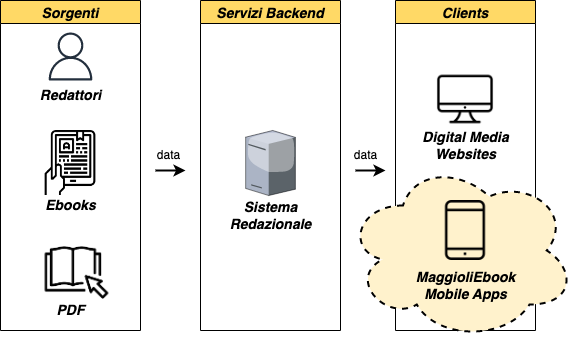
\includegraphics[width=0.7\textwidth]{img/contesto-aziendale.png}
    \end{figure}
    \begin{itemize}
        \item Core Business: servizi per la pubblica amministrazione e professionisti
        \item Dominio dell'editoria digitale
        \item Necessità di sviluppare un nuovo metodo di accesso alle pubblicazioni digitali che sia più accessibile e pratico
    \end{itemize}
\end{frame}

\begin{frame}{Requisiti: Processo}
    
\end{frame}

\begin{frame}
    \begin{figure}[H]
        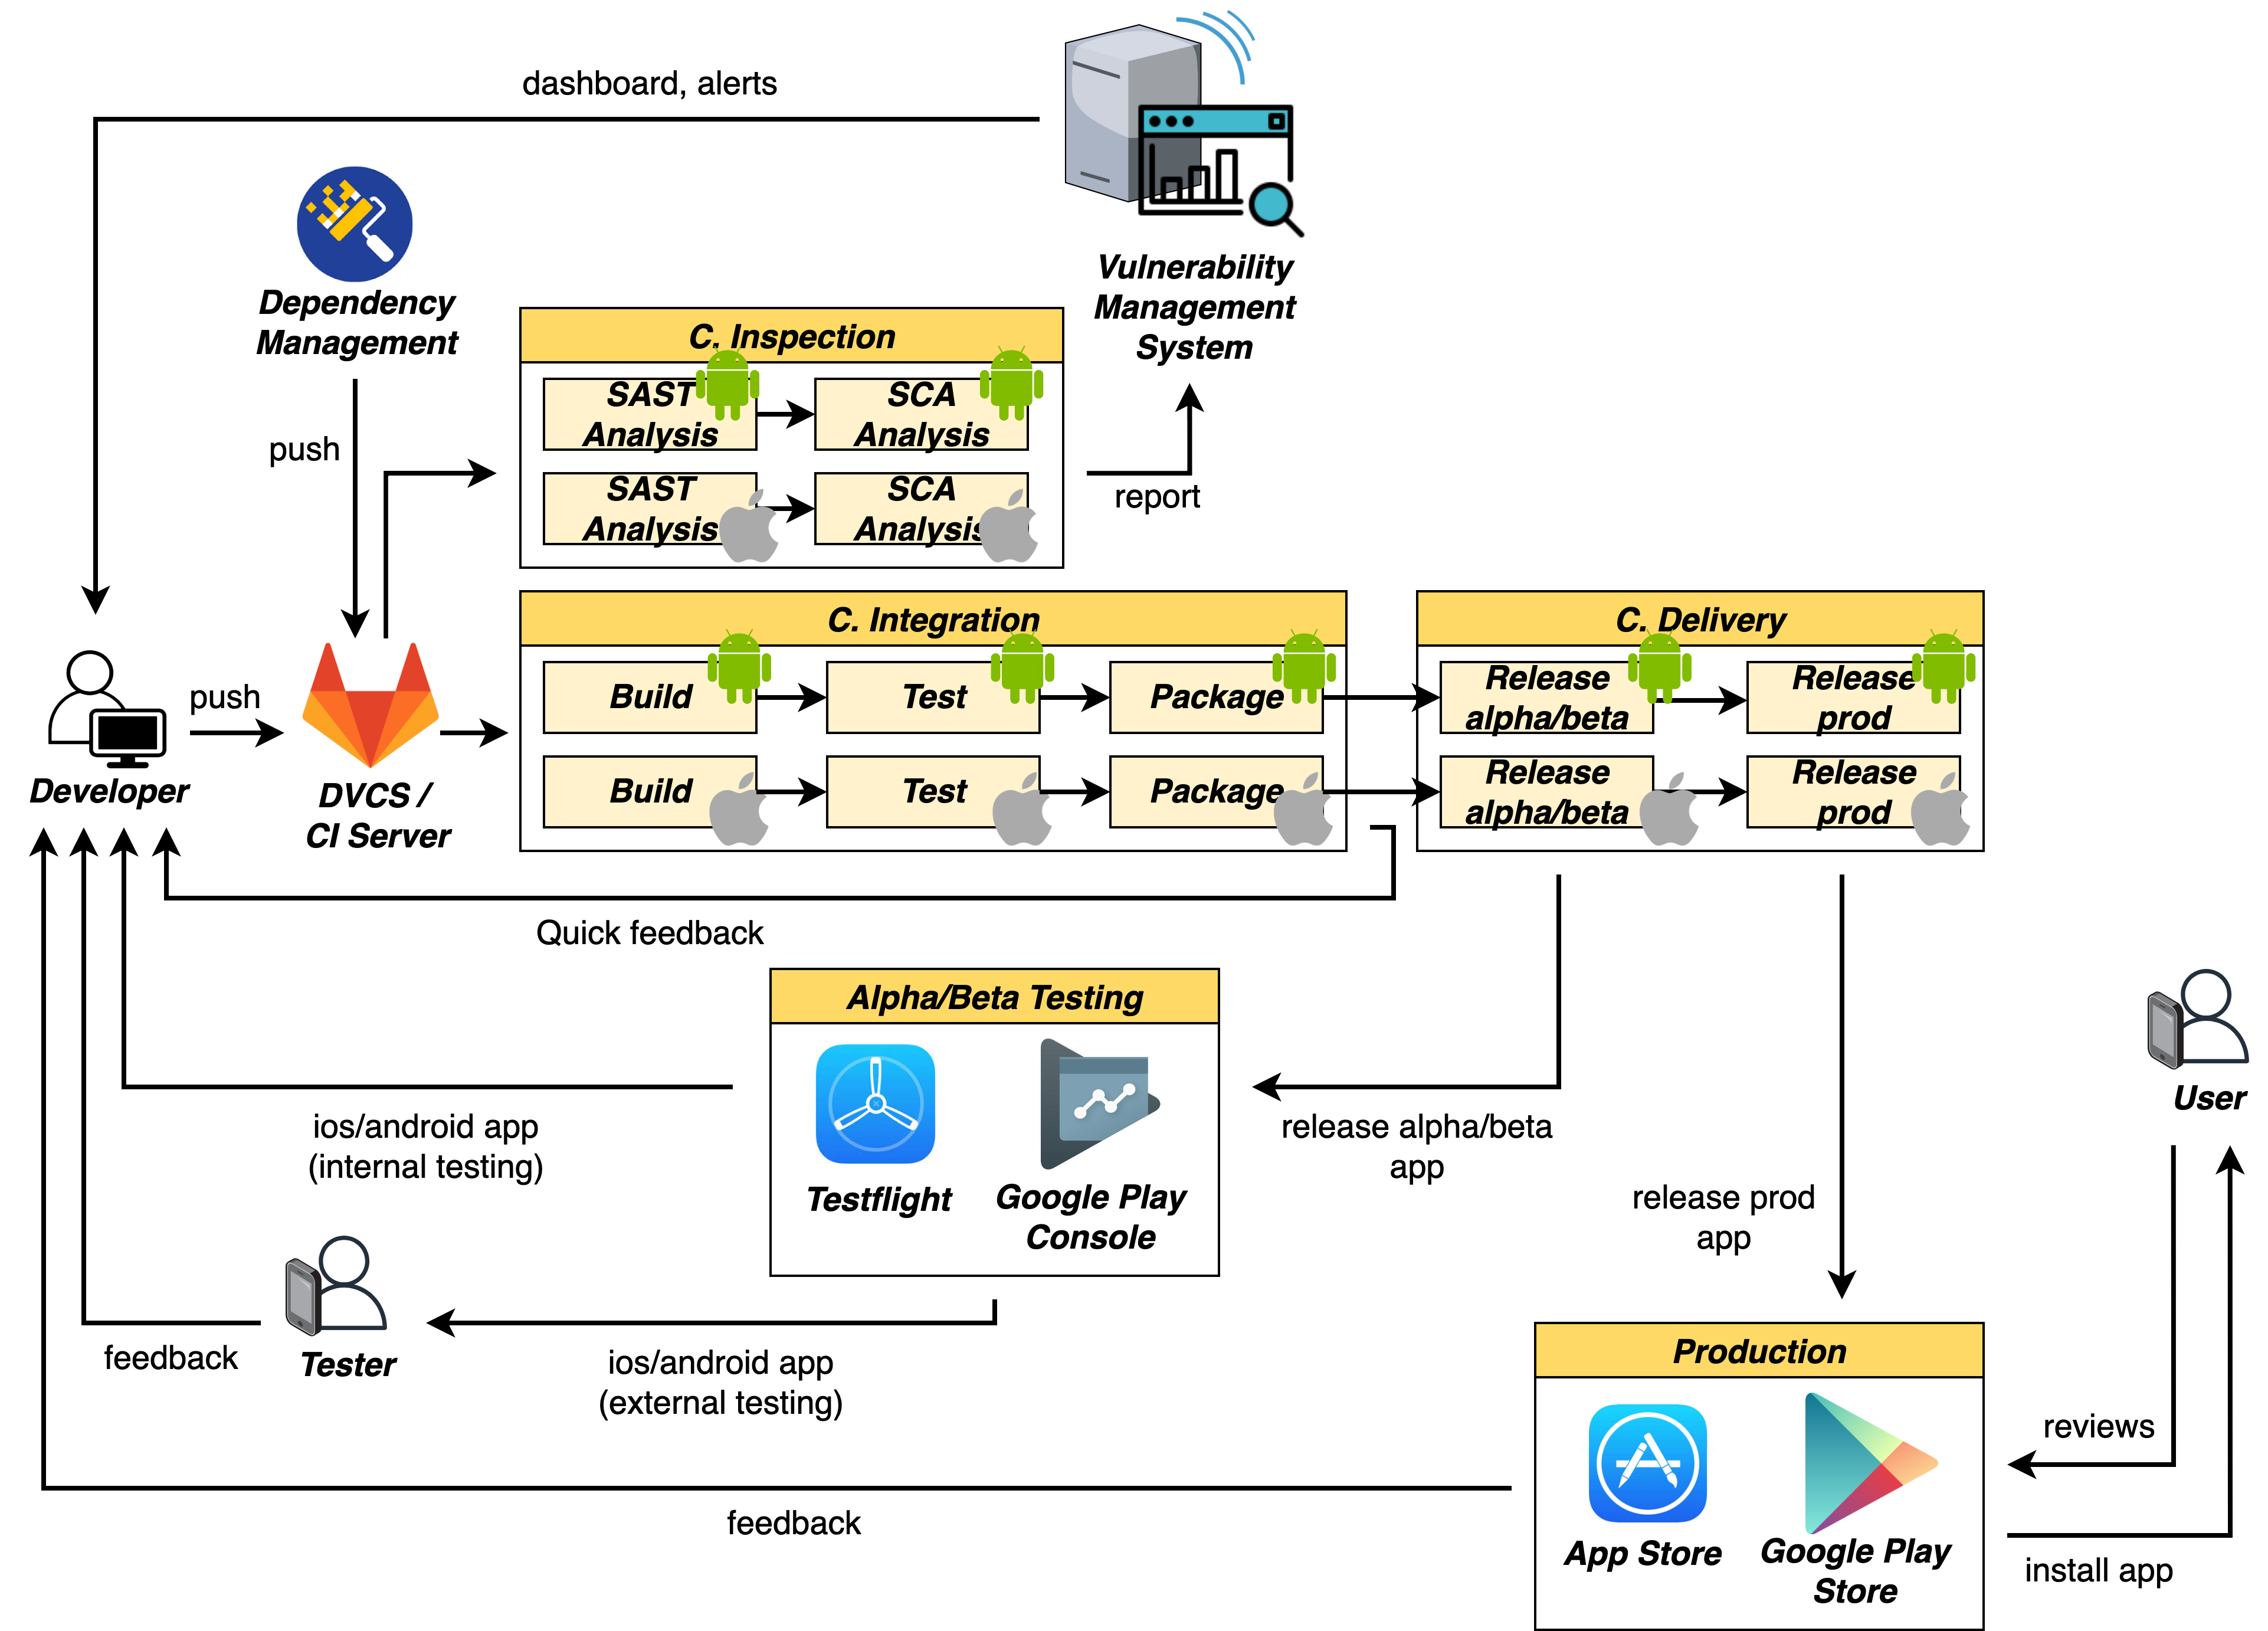
\includegraphics[width=0.82\textwidth]{img/full-cicd.png}
    \end{figure}
\end{frame}

\begin{frame}{Requisiti: Applicazione}

\end{frame}